\documentclass[11pt, oneside]{article} 
\usepackage{geometry}
\geometry{letterpaper} 
\usepackage{graphicx}
	
\usepackage{amssymb}
\usepackage{amsmath}
\usepackage{parskip}
\usepackage{color}
\usepackage{hyperref}

\graphicspath{{/Users/telliott/Github/calculus_book/png/}}
% \begin{center} 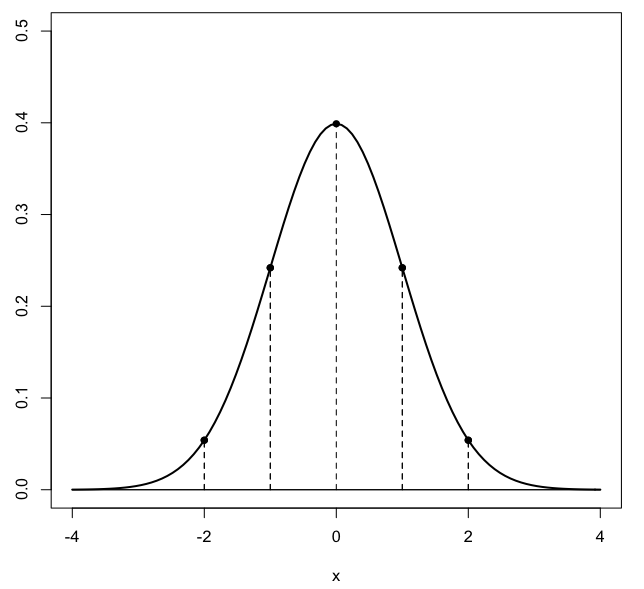
\includegraphics [scale=0.4] {gauss3.png} \end{center}

\title{More induction}
\date{}

\begin{document}
\maketitle
\Large

Previously showed that the sum of integers
\[ sum_{k=1}^{k=n} = \frac{1}{2} \cdot n(n+1) \]

We showed this "proof without words":

\begin{center} 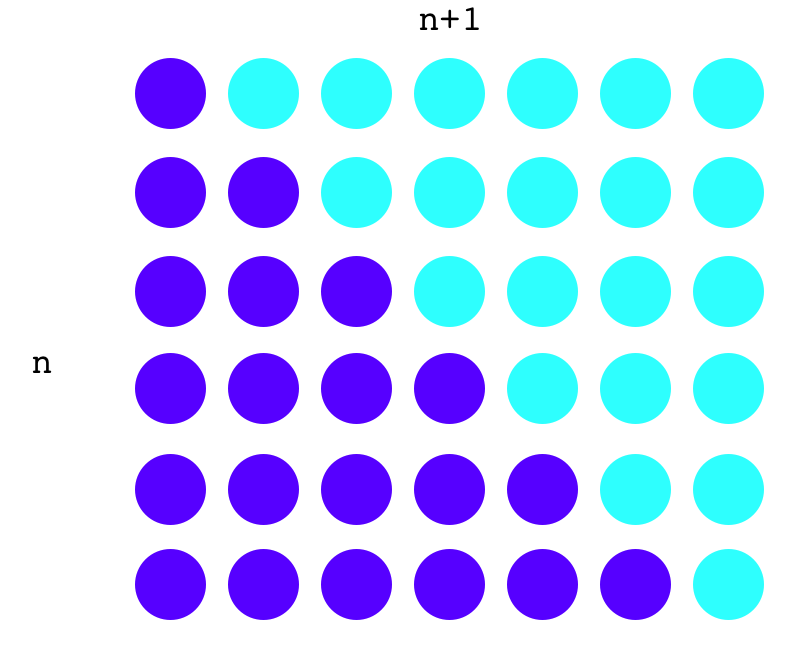
\includegraphics [scale=0.25] {sum_n.png}\end{center}

\subsection*{Derivation using sums}
It seems a shame to spoil such a beautiful proof as the one above,  let alone the inductive proof,  by saying anything more, but I can't resist.  

You will notice that we were given the formula and only proved it true.  As we quoted Archimedes in the first chapter

\begin{quote}it is of course easier, when we have previously acquired by the method some knowledge of questions, to supply the proof than it is to find the proof without any previous knowledge.\end{quote}

I'd like to derive the equation we have been using using algebra.  The general method can be used to get the sum of the squares of integers, or their cubes, or even higher powers.

For any number $k$ it is true that
\[ (k+1)^2 = k^2 + 2k + 1 \]
So consider what happens if we sum the values from $k=1 \rightarrow n$ for each of these terms
\[ \sum_{k=1}^n (k+1)^2 = \sum_{k=1}^n k^2 + \sum_{k=1}^n 2k + \sum_{k=1}^n 1 \]

If the equation is valid for any individual $k$, then it is also true adding the equations for all $k$ from $1$ up to $n$.

Rearranging
\[ \sum_{k=1}^n (k+1)^2 - \sum_{k=1}^n k^2 = \sum_{k=1}^n 2k + \sum_{k=1}^n 1 \]
Now think about the left-hand side in our equation. 
\[ \sum_{k=1}^n (k+1)^2 - \sum_{k=1}^n k^2 \]
If we count down rather than up, start with $k=n$.  We have the following terms
\[ k = n \ \ \text{gives} \ \ (n+1)^2 - (n)^2 \]
\[ k = n-1 \ \ \text{gives} \ \ (n)^2 - (n-1)^2 \]
\[ k = n-2 \ \ \text{gives} \ \  (n-1)^2 - (n-2)^2 \]
\[ \cdots \]
\[ k = 1 \rightarrow \ \ (2)^2 - (1)^2 \]

We must add all of these together.  But notice how all the terms except the first and last cancel.  For example we have $-(n)^2$ in the top line and $(n)^2$ in the second. This is called a "collapsing" or "telescoping" sum.  We obtain
\[ S = (n+1)^2 - 1 \]\

Bringing back the right-hand side  we have
\[ (n+1)^2 - 1 = \sum_{k=1}^n 2k + \sum_{k=1}^n 1 \]

We can bring the constant factor $2$ out of the sum, and also, we recognize that the sum of the value $1$ a total of $n$ times is just $n$.
\[ (n+1)^2 - 1 = 2\sum_{k=1}^n k + n \]

Subtract $n$ from both sides.  The left hand side is
\[ (n+1)^2 - 1 - n = n^2 + n = n(n+1) \]
Finally, divide by $2$:
\[ \sum_{k=1}^n k = \frac{n (n+1)}{2} \]
That's our formula.

There is much more (sum of squares, cubes and so on) in the next chapter.
\subsection*{Odd number theorem}

Here is a simple but very useful inductive proof.

The \emph{odd number theorem} says that the sum of the first $n$ odd numbers is equal to $n^2$.  Here is a "proof without words".

\begin{center} 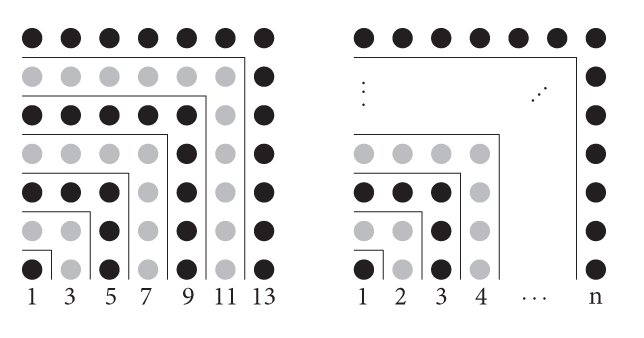
\includegraphics [scale=0.4] {odd_number_theorem.png} \end{center}

We prove this by induction.

\[ \ (0 \times 2 + 1) +  (1 \times 2 + 1) + (2 \times 2 + 1) + (\dots \]
\[ \dots + (n-1) \times 2 + 1) = n^2 \]

Notice that the $n$th odd number is $2 \times (n-1) + 1$.

Our formula says that
\[ 1 + 3 + 5 + \dots + (2n - 1) = n^2 \]
If you like the summation style:
\[ \sum_{k=0}^n 2k - 1 = k^2 \]

As an example, the first five odd numbers are
\[ 1 + 3 + 5 + 7 + 9 = 25 = 5^2 \]

So, if we consider the next odd number, $n$ changes to $n+1$.  The left-hand side gets another term:  we add $2 \times (n+1)-1$ to it.  That is equal to $2n + 1$.

To maintain the equality, add the same quantity to the right-hand side:
\[ n^2 + 2n + 1 = (n+1)^2 \]
Rearrange the result, and that's our formula back again.  We have proved the inductive step.  

To finish, note that the base case is simply
\[ 1 = 1^2 \]
$\square$

\end{document}  